\chapter{Virtualisatie}
\label{ch:virtualisatie}

In dit hoofdstuk zal bekeken worden waarom en hoe virtualisatie ontstaan is. Verder zal bekeken worden welke concepten meespelen binnen virtualisatie. Dit hoofdstuk dient als een inleiding om concepten zoals software containers, unikernels en virtuele machines te kunnen begrijpen.

In de jaren 60 was de tijd dat een computer kon gebruikt worden beperkt (\cite{conferences_modern_1968}). Bij de eerste computers, had men problemen om programma's uit te werken. Dit lag vooral aan de tijd dat er kon gewerkt worden aan de computer en de weinige computers die beschikbaar waren. Een voorbeeld van het ontwikkelen van een programma in die tijd was het volgende: "De broncode van het programma werd ingegeven en in een wachtrij geplaatst. Pas een bepaalde tijd later konden de resultaten van het programma bekeken worden. Fouten in het geschreven programma zorgden voor veel tijdsverlies." (\cite{conferences_modern_1968})

Eén van de grootste bijdrages, tot de ontwikkelingssnelheid van programma's, is de lengte van de feedbackcyclus: hoe snel kan een programma getest worden wanneer er een verandering in de broncode plaatsvindt. Als er lang moet worden gewacht op de feedback, dan kan dit tijdsverlies tot gevolg hebben.

Timesharing (\cite{pyke_jr._time-shared_1967}) werd uitgevonden om het verlies van tijd, tijdens het ontwikkelen van programma's, te beperken. Bij timesharing kunnen gebruikers inloggen op een console en zo met meerdere tegelijk van de computer gebruik maken. Dit was een technische uitdaging. Elke gebruiker en zijn programma's bevinden zich binnen een afzonderlijke context bij timesharing. De computer moet van de ene context naar de andere kunnen veranderen. Timesharing zou de basis vormen voor het moderne besturingssysteem. Eén van de moeilijkheden van timesharing is de isolatie van de verschillende processen en gebruikers. De processen moeten zich bevinden binnen een verschillende context om geen invloed op elkaar te hebben.

Doorheen de tijd kregen computers meer middelen ter beschikking. De meeste programma's konden niet langer alle middelen van de computer benutten. Dit zorgde voor de creatie van virtuele middelen of virtual resources (\cite{vakilinia_modeling_2015}). Om deze virtuele middelen te voorzien moeten bepaalde delen van de computer gevirtualiseerd worden. Dit kan voorkomen onder verschillende vormen zoals hardware virtualisatie en virtualisatie van het besturingssysteem.

\begin{wrapfigure}{r}{0.3\textwidth}
    \centering
    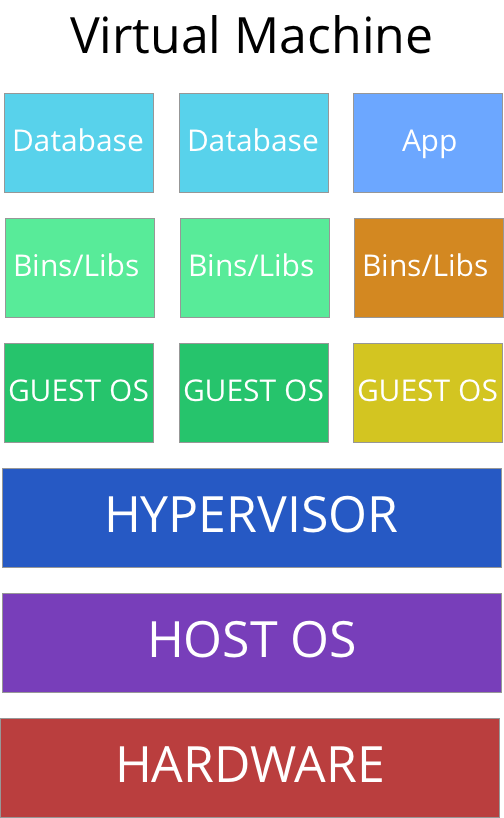
\includegraphics[width=3cm]{img/virtual-machine}
    \caption{structuur van een virtuele machine}
    \label{fig:virtualmachine}
\end{wrapfigure}

Het concept van virtualisatie deelt een aantal gelijkenissen met timesharing. De computer wordt opgedeeld in verschillende delen bij virtualisatie. Bij timesharing wordt de computer opgedeeld in afzonderlijke contexten.

Een aantal voordelen van virtualisatie zijn de volgende: financieel voordeel (men kan van één taak naar meerdere taken gaan op één computer), het besparen van energie (\cite{beloglazov_energy_2010}) en veiligheid(\cite{mortleman_security_2009}).

Een virtuele machine (\cite{smith_architecture_2005}) bootst een computer na. Een virtuele machine kan de middelen van de fysieke computer, waar het zich op bevindt, gebruiken. Dit zorgt ervoor dat de middelen van de fysieke computer kunnen gebruikt worden als virtuele middelen. Doorheen deze bachelorproef zal naar de fysieke computer verwezen worden als de host machine. Guest is de naam dat wordt gegeven aan virtuele machines die zich bevinden op de host. In het volgende deel zullen we de laag tussen de host machine en virtuele machine bekijken: de hypervisor. Figuur \ref{fig:virtualmachine} toont de structuur van een virtuele machine. 

\section{Hypervisor}

Een hypervisor (\cite{popek_formal_1974}) is een voorbeeld van hardware virtualisatie. Het is een stuk software, firmware of hardware, dat de laag vormt tussen de virtuele machine en de host machine. De host machine zorgt voor de middelen zoals CPU, RAM, enzoverder. Elke virtuele machine die zich bevindt op de host machine zal dan gebruik kunnen maken van een gedeelte van deze middelen. Doordat virtualisatie alomtegenwoordig geworden is in datacenters (\cite{soundararajan_impact_2010}) heeft het ervoor gezorgd dat er meer logica komt te liggen bij de hypervisor. De hypervisor neemt verder de rol op zich van het verdelen van de middelen en het beheren van de guests. Er zijn twee soorten hypervisors: type 1 en type 2. Type 1 is de bare-metal hypervisor en type 2 de hosted hypervisor.

\newpage

\subsection{Hosted Hypervisors}

\begin{wrapfigure}{r}{0.3\textwidth}
    \centering
    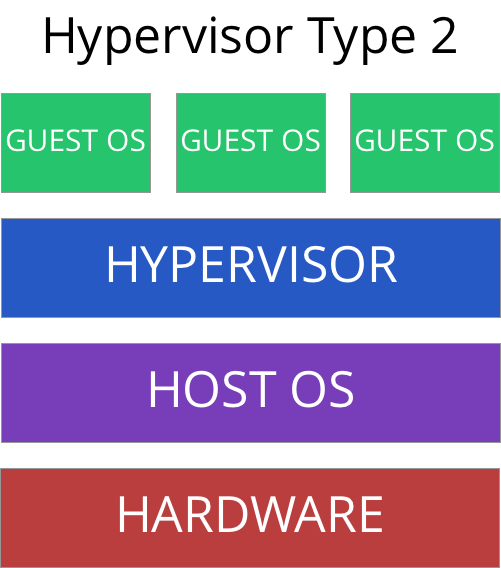
\includegraphics[width=3cm]{img/hypervisor-2}
    \caption{structuur van een hosted hypervisor}
    \label{fig:hypervisor-2}
\end{wrapfigure}

Als eerste zullen we de hosted hypervisor of type 2 hypervisor behandelen. Figuur \ref{fig:hypervisor-2} toont de structuur van een hosted hypervisor. De hosted hypervisor bevindt zich op het besturingssysteem van de host machine en heeft geen directe toegang tot de hardware. De type 2 hypervisor is dus compleet afhankelijk van het besturingssysteem van de host om zijn taken uit te voeren. Als er problemen optreden in het besturingssysteem van de host heeft dit gevolgen voor de hypervisor en guests.

Voorbeelden van hosted hypervisors zijn: Oracle Virtualbox (\cite{oracle_oracle_2016}) en VMware Workstation (\cite{vmware_vmware_2016}).

\subsection{Bare-metal Hypervisors}

\begin{wrapfigure}{l}{0.3\textwidth}
    \centering
    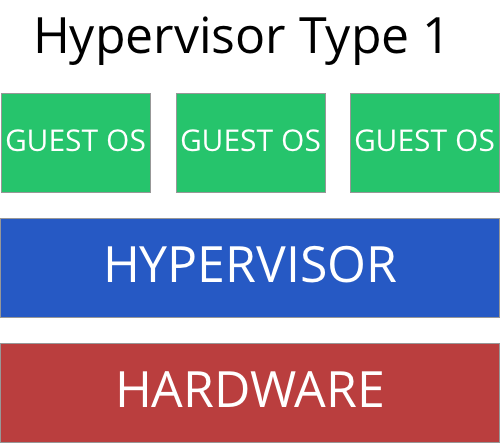
\includegraphics[width=3cm]{img/hypervisor-1}
    \caption{structuur van een bare-metal hypervisor}
    \label{fig:hypervisor-1}
\end{wrapfigure}

Type 1, bare-metal, embedded of native hypervisors bevinden zich rechtstreeks op de hardware. De voornaamste taak van de hypervisor is het beheren en verdelen van middelen. Dit maakt de hardware hypervisor kleiner in omvang dan de hosted hypervisor. De hosted hypervisor is niet afhankelijk van het besturingssysteem van de host machine want de hosted hypervisor bevindt zich rechtstreeks op de hardware. Figuur \ref{fig:hypervisor-1} toont de structuur van een bare-metal hypervisor.

Er is een laag minder in de structuur dus dit betekent dat er minder instructies moeten worden uitgevoerd bij een bepaalde handeling. Dit heeft een betere prestatie tot gevolg. Omdat er geen problemen kunnen zijn met het besturingssysteem van de host kan er aangenomen worden dat deze soort hypervisors stabieler zijn. Wanneer het besturingssysteem van de host faalt bij een hosted hypervisor dan zal dit gevolgen hebben voor de guests.

Een paar voorbeelden van bare-metal hypervisors zijn VMware ESXi en Xen.

\section{Operating System-level Virtualisation}

Naast hardware virtualisatie kan ook een besturingssysteem gevirtualiseerd worden. Bij deze toepassing van virtualisatie worden de mogelijkheden van de kernel gebruikt. De kernel van bepaalde besturingssystemen laat toe om meerdere geïsoleerde namespaces tegelijkertijd te laten werken. Dit zorgt ervoor dat er maar één besturingssysteem moet zijn om verschillende programma's naast elkaar en geïsoleerd te laten werken.

Elke namespace heeft zijn eigen configuratie en zijn geïsoleerd van elkaar. Dit geeft eveneens de beperking dat de guests over een besturingssysteem of kernel moeten beschikken, die overeenkomt met de host.

Tegenover hardware virtualisatie zal besturingssysteem virtualisatie minder gebruik maken van middelen omdat er maar één besturingssysteem is. Dit is omdat het besturingssysteem wordt gedeeld. Dit geeft voordelen bij de prestatie.

Voorbeelden van besturingssysteem virtualisatie zijn: chroot (\cite{linux_chroot2_????}), Solaris Containers (\cite{oracle_solaris_2016}) en Docker (\cite{docker_docker_2016}).

Besturingssysteem virtualisatie is vooral bekend geworden door Docker vanaf 2013 (\cite{hykes_future_2013}). In het volgende hoofdstuk wordt verder ingegaan op besturingssysteem virtualisatie onder de vorm van software containers.
